% Created by tikzDevice version 0.6.2-92-0ad2792 on 2013-05-05 16:12:43
% !TEX encoding = UTF-8 Unicode
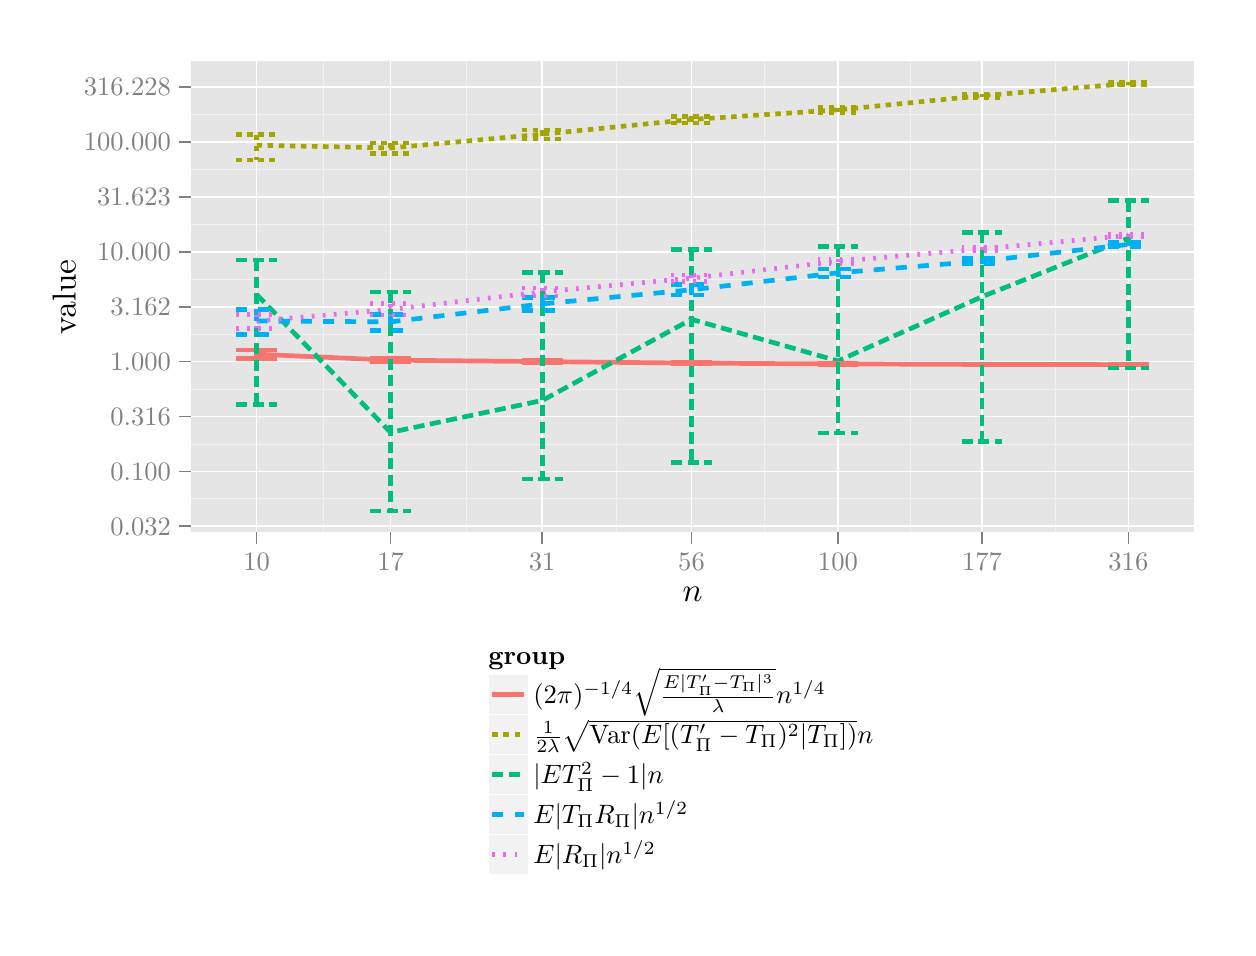
\begin{tikzpicture}[x=1pt,y=1pt]
\definecolor[named]{fillColor}{rgb}{1.00,1.00,1.00}
\path[use as bounding box,fill=fillColor,fill opacity=0.00] (0,0) rectangle (433.62,325.21);
\begin{scope}
\path[clip] (  0.00,  0.00) rectangle (433.62,325.21);
\definecolor[named]{drawColor}{rgb}{1.00,1.00,1.00}
\definecolor[named]{fillColor}{rgb}{1.00,1.00,1.00}

\path[draw=drawColor,line width= 0.6pt,line join=round,line cap=round,fill=fillColor] (  0.00,  0.00) rectangle (433.62,325.21);
\end{scope}
\begin{scope}
\path[clip] ( 58.88,142.81) rectangle (421.57,313.17);
\definecolor[named]{fillColor}{rgb}{0.90,0.90,0.90}

\path[fill=fillColor] ( 58.88,142.81) rectangle (421.57,313.17);
\definecolor[named]{drawColor}{rgb}{0.95,0.95,0.95}

\path[draw=drawColor,line width= 0.3pt,line join=round] ( 58.88,154.98) --
	(421.57,154.98);

\path[draw=drawColor,line width= 0.3pt,line join=round] ( 58.88,174.73) --
	(421.57,174.73);

\path[draw=drawColor,line width= 0.3pt,line join=round] ( 58.88,194.60) --
	(421.57,194.60);

\path[draw=drawColor,line width= 0.3pt,line join=round] ( 58.88,214.46) --
	(421.57,214.46);

\path[draw=drawColor,line width= 0.3pt,line join=round] ( 58.88,234.32) --
	(421.57,234.32);

\path[draw=drawColor,line width= 0.3pt,line join=round] ( 58.88,254.18) --
	(421.57,254.18);

\path[draw=drawColor,line width= 0.3pt,line join=round] ( 58.88,274.04) --
	(421.57,274.04);

\path[draw=drawColor,line width= 0.3pt,line join=round] ( 58.88,293.91) --
	(421.57,293.91);

\path[draw=drawColor,line width= 0.3pt,line join=round] (106.92,142.81) --
	(106.92,313.17);

\path[draw=drawColor,line width= 0.3pt,line join=round] (158.53,142.81) --
	(158.53,313.17);

\path[draw=drawColor,line width= 0.3pt,line join=round] (212.91,142.81) --
	(212.91,313.17);

\path[draw=drawColor,line width= 0.3pt,line join=round] (266.33,142.81) --
	(266.33,313.17);

\path[draw=drawColor,line width= 0.3pt,line join=round] (318.82,142.81) --
	(318.82,313.17);

\path[draw=drawColor,line width= 0.3pt,line join=round] (371.30,142.81) --
	(371.30,313.17);
\definecolor[named]{drawColor}{rgb}{1.00,1.00,1.00}

\path[draw=drawColor,line width= 0.6pt,line join=round] ( 58.88,145.15) --
	(421.57,145.15);

\path[draw=drawColor,line width= 0.6pt,line join=round] ( 58.88,164.81) --
	(421.57,164.81);

\path[draw=drawColor,line width= 0.6pt,line join=round] ( 58.88,184.66) --
	(421.57,184.66);

\path[draw=drawColor,line width= 0.6pt,line join=round] ( 58.88,204.53) --
	(421.57,204.53);

\path[draw=drawColor,line width= 0.6pt,line join=round] ( 58.88,224.39) --
	(421.57,224.39);

\path[draw=drawColor,line width= 0.6pt,line join=round] ( 58.88,244.25) --
	(421.57,244.25);

\path[draw=drawColor,line width= 0.6pt,line join=round] ( 58.88,264.11) --
	(421.57,264.11);

\path[draw=drawColor,line width= 0.6pt,line join=round] ( 58.88,283.97) --
	(421.57,283.97);

\path[draw=drawColor,line width= 0.6pt,line join=round] ( 58.88,303.84) --
	(421.57,303.84);

\path[draw=drawColor,line width= 0.6pt,line join=round] ( 82.72,142.81) --
	( 82.72,313.17);

\path[draw=drawColor,line width= 0.6pt,line join=round] (131.13,142.81) --
	(131.13,313.17);

\path[draw=drawColor,line width= 0.6pt,line join=round] (185.93,142.81) --
	(185.93,313.17);

\path[draw=drawColor,line width= 0.6pt,line join=round] (239.88,142.81) --
	(239.88,313.17);

\path[draw=drawColor,line width= 0.6pt,line join=round] (292.78,142.81) --
	(292.78,313.17);

\path[draw=drawColor,line width= 0.6pt,line join=round] (344.86,142.81) --
	(344.86,313.17);

\path[draw=drawColor,line width= 0.6pt,line join=round] (397.74,142.81) --
	(397.74,313.17);
\definecolor[named]{drawColor}{rgb}{0.97,0.46,0.43}

\path[draw=drawColor,line width= 1.7pt,line join=round] ( 82.72,207.22) --
	(131.13,205.06) --
	(185.93,204.54) --
	(239.88,203.99) --
	(292.78,203.69) --
	(344.86,203.53) --
	(397.74,203.44);
\definecolor[named]{drawColor}{rgb}{0.64,0.65,0.00}

\path[draw=drawColor,line width= 1.7pt,dash pattern=on 2pt off 2pt ,line join=round] ( 82.72,282.74) --
	(131.13,281.74) --
	(185.93,286.71) --
	(239.88,292.04) --
	(292.78,295.51) --
	(344.86,300.63) --
	(397.74,305.03);
\definecolor[named]{drawColor}{rgb}{0.00,0.75,0.49}

\path[draw=drawColor,line width= 1.7pt,dash pattern=on 4pt off 2pt ,line join=round] ( 82.72,228.83) --
	(131.13,178.97) --
	(185.93,190.49) --
	(239.88,219.83) --
	(292.78,204.78) --
	(344.86,227.98) --
	(397.74,249.14);
\definecolor[named]{drawColor}{rgb}{0.00,0.69,0.96}

\path[draw=drawColor,line width= 1.7pt,dash pattern=on 4pt off 4pt ,line join=round] ( 82.72,219.20) --
	(131.13,218.91) --
	(185.93,225.39) --
	(239.88,230.50) --
	(292.78,236.62) --
	(344.86,240.89) --
	(397.74,246.87);
\definecolor[named]{drawColor}{rgb}{0.91,0.42,0.95}

\path[draw=drawColor,line width= 1.7pt,dash pattern=on 1pt off 3pt ,line join=round] ( 82.72,219.21) --
	(131.13,223.37) --
	(185.93,229.76) --
	(239.88,234.70) --
	(292.78,240.75) --
	(344.86,245.25) --
	(397.74,250.15);
\definecolor[named]{drawColor}{rgb}{0.97,0.46,0.43}

\path[draw=drawColor,line width= 1.7pt,line join=round] ( 75.37,208.70) --
	( 90.07,208.70);

\path[draw=drawColor,line width= 1.7pt,line join=round] ( 82.72,208.70) --
	( 82.72,205.69);

\path[draw=drawColor,line width= 1.7pt,line join=round] ( 75.37,205.69) --
	( 90.07,205.69);

\path[draw=drawColor,line width= 1.7pt,line join=round] (123.78,205.74) --
	(138.48,205.74);

\path[draw=drawColor,line width= 1.7pt,line join=round] (131.13,205.74) --
	(131.13,204.43);

\path[draw=drawColor,line width= 1.7pt,line join=round] (123.78,204.43) --
	(138.48,204.43);

\path[draw=drawColor,line width= 1.7pt,line join=round] (178.58,204.92) --
	(193.28,204.92);

\path[draw=drawColor,line width= 1.7pt,line join=round] (185.93,204.92) --
	(185.93,204.16);

\path[draw=drawColor,line width= 1.7pt,line join=round] (178.58,204.16) --
	(193.28,204.16);

\path[draw=drawColor,line width= 1.7pt,line join=round] (232.53,204.22) --
	(247.23,204.22);

\path[draw=drawColor,line width= 1.7pt,line join=round] (239.88,204.22) --
	(239.88,203.78);

\path[draw=drawColor,line width= 1.7pt,line join=round] (232.53,203.78) --
	(247.23,203.78);

\path[draw=drawColor,line width= 1.7pt,line join=round] (285.42,203.81) --
	(300.13,203.81);

\path[draw=drawColor,line width= 1.7pt,line join=round] (292.78,203.81) --
	(292.78,203.59);

\path[draw=drawColor,line width= 1.7pt,line join=round] (285.42,203.59) --
	(300.13,203.59);

\path[draw=drawColor,line width= 1.7pt,line join=round] (337.51,203.60) --
	(352.22,203.60);

\path[draw=drawColor,line width= 1.7pt,line join=round] (344.86,203.60) --
	(344.86,203.47);

\path[draw=drawColor,line width= 1.7pt,line join=round] (337.51,203.47) --
	(352.22,203.47);

\path[draw=drawColor,line width= 1.7pt,line join=round] (390.39,203.48) --
	(405.09,203.48);

\path[draw=drawColor,line width= 1.7pt,line join=round] (397.74,203.48) --
	(397.74,203.40);

\path[draw=drawColor,line width= 1.7pt,line join=round] (390.39,203.40) --
	(405.09,203.40);
\definecolor[named]{drawColor}{rgb}{0.64,0.65,0.00}

\path[draw=drawColor,line width= 1.7pt,dash pattern=on 2pt off 2pt ,line join=round] ( 75.37,286.54) --
	( 90.07,286.54);

\path[draw=drawColor,line width= 1.7pt,dash pattern=on 2pt off 2pt ,line join=round] ( 82.72,286.54) --
	( 82.72,277.38);

\path[draw=drawColor,line width= 1.7pt,dash pattern=on 2pt off 2pt ,line join=round] ( 75.37,277.38) --
	( 90.07,277.38);

\path[draw=drawColor,line width= 1.7pt,dash pattern=on 2pt off 2pt ,line join=round] (123.78,283.55) --
	(138.48,283.55);

\path[draw=drawColor,line width= 1.7pt,dash pattern=on 2pt off 2pt ,line join=round] (131.13,283.55) --
	(131.13,279.65);

\path[draw=drawColor,line width= 1.7pt,dash pattern=on 2pt off 2pt ,line join=round] (123.78,279.65) --
	(138.48,279.65);

\path[draw=drawColor,line width= 1.7pt,dash pattern=on 2pt off 2pt ,line join=round] (178.58,288.22) --
	(193.28,288.22);

\path[draw=drawColor,line width= 1.7pt,dash pattern=on 2pt off 2pt ,line join=round] (185.93,288.22) --
	(185.93,285.03);

\path[draw=drawColor,line width= 1.7pt,dash pattern=on 2pt off 2pt ,line join=round] (178.58,285.03) --
	(193.28,285.03);

\path[draw=drawColor,line width= 1.7pt,dash pattern=on 2pt off 2pt ,line join=round] (232.53,293.18) --
	(247.23,293.18);

\path[draw=drawColor,line width= 1.7pt,dash pattern=on 2pt off 2pt ,line join=round] (239.88,293.18) --
	(239.88,290.76);

\path[draw=drawColor,line width= 1.7pt,dash pattern=on 2pt off 2pt ,line join=round] (232.53,290.76) --
	(247.23,290.76);

\path[draw=drawColor,line width= 1.7pt,dash pattern=on 2pt off 2pt ,line join=round] (285.42,296.28) --
	(300.13,296.28);

\path[draw=drawColor,line width= 1.7pt,dash pattern=on 2pt off 2pt ,line join=round] (292.78,296.28) --
	(292.78,294.66);

\path[draw=drawColor,line width= 1.7pt,dash pattern=on 2pt off 2pt ,line join=round] (285.42,294.66) --
	(300.13,294.66);

\path[draw=drawColor,line width= 1.7pt,dash pattern=on 2pt off 2pt ,line join=round] (337.51,301.23) --
	(352.22,301.23);

\path[draw=drawColor,line width= 1.7pt,dash pattern=on 2pt off 2pt ,line join=round] (344.86,301.23) --
	(344.86,300.04);

\path[draw=drawColor,line width= 1.7pt,dash pattern=on 2pt off 2pt ,line join=round] (337.51,300.04) --
	(352.22,300.04);

\path[draw=drawColor,line width= 1.7pt,dash pattern=on 2pt off 2pt ,line join=round] (390.39,305.43) --
	(405.09,305.43);

\path[draw=drawColor,line width= 1.7pt,dash pattern=on 2pt off 2pt ,line join=round] (397.74,305.43) --
	(397.74,304.62);

\path[draw=drawColor,line width= 1.7pt,dash pattern=on 2pt off 2pt ,line join=round] (390.39,304.62) --
	(405.09,304.62);
\definecolor[named]{drawColor}{rgb}{0.00,0.75,0.49}

\path[draw=drawColor,line width= 1.7pt,dash pattern=on 4pt off 2pt ,line join=round] ( 75.37,241.29) --
	( 90.07,241.29);

\path[draw=drawColor,line width= 1.7pt,dash pattern=on 4pt off 2pt ,line join=round] ( 82.72,241.29) --
	( 82.72,188.99);

\path[draw=drawColor,line width= 1.7pt,dash pattern=on 4pt off 2pt ,line join=round] ( 75.37,188.99) --
	( 90.07,188.99);

\path[draw=drawColor,line width= 1.7pt,dash pattern=on 4pt off 2pt ,line join=round] (123.78,229.66) --
	(138.48,229.66);

\path[draw=drawColor,line width= 1.7pt,dash pattern=on 4pt off 2pt ,line join=round] (131.13,229.66) --
	(131.13,150.56);

\path[draw=drawColor,line width= 1.7pt,dash pattern=on 4pt off 2pt ,line join=round] (123.78,150.56) --
	(138.48,150.56);

\path[draw=drawColor,line width= 1.7pt,dash pattern=on 4pt off 2pt ,line join=round] (178.58,236.84) --
	(193.28,236.84);

\path[draw=drawColor,line width= 1.7pt,dash pattern=on 4pt off 2pt ,line join=round] (185.93,236.84) --
	(185.93,162.12);

\path[draw=drawColor,line width= 1.7pt,dash pattern=on 4pt off 2pt ,line join=round] (178.58,162.12) --
	(193.28,162.12);

\path[draw=drawColor,line width= 1.7pt,dash pattern=on 4pt off 2pt ,line join=round] (232.53,244.94) --
	(247.23,244.94);

\path[draw=drawColor,line width= 1.7pt,dash pattern=on 4pt off 2pt ,line join=round] (239.88,244.94) --
	(239.88,168.10);

\path[draw=drawColor,line width= 1.7pt,dash pattern=on 4pt off 2pt ,line join=round] (232.53,168.10) --
	(247.23,168.10);

\path[draw=drawColor,line width= 1.7pt,dash pattern=on 4pt off 2pt ,line join=round] (285.42,246.23) --
	(300.13,246.23);

\path[draw=drawColor,line width= 1.7pt,dash pattern=on 4pt off 2pt ,line join=round] (292.78,246.23) --
	(292.78,178.72);

\path[draw=drawColor,line width= 1.7pt,dash pattern=on 4pt off 2pt ,line join=round] (285.42,178.72) --
	(300.13,178.72);

\path[draw=drawColor,line width= 1.7pt,dash pattern=on 4pt off 2pt ,line join=round] (337.51,251.29) --
	(352.22,251.29);

\path[draw=drawColor,line width= 1.7pt,dash pattern=on 4pt off 2pt ,line join=round] (344.86,251.29) --
	(344.86,175.75);

\path[draw=drawColor,line width= 1.7pt,dash pattern=on 4pt off 2pt ,line join=round] (337.51,175.75) --
	(352.22,175.75);

\path[draw=drawColor,line width= 1.7pt,dash pattern=on 4pt off 2pt ,line join=round] (390.39,262.73) --
	(405.09,262.73);

\path[draw=drawColor,line width= 1.7pt,dash pattern=on 4pt off 2pt ,line join=round] (397.74,262.73) --
	(397.74,202.27);

\path[draw=drawColor,line width= 1.7pt,dash pattern=on 4pt off 2pt ,line join=round] (390.39,202.27) --
	(405.09,202.27);
\definecolor[named]{drawColor}{rgb}{0.00,0.69,0.96}

\path[draw=drawColor,line width= 1.7pt,dash pattern=on 4pt off 4pt ,line join=round] ( 75.37,223.38) --
	( 90.07,223.38);

\path[draw=drawColor,line width= 1.7pt,dash pattern=on 4pt off 4pt ,line join=round] ( 82.72,223.38) --
	( 82.72,214.35);

\path[draw=drawColor,line width= 1.7pt,dash pattern=on 4pt off 4pt ,line join=round] ( 75.37,214.35) --
	( 90.07,214.35);

\path[draw=drawColor,line width= 1.7pt,dash pattern=on 4pt off 4pt ,line join=round] (123.78,221.64) --
	(138.48,221.64);

\path[draw=drawColor,line width= 1.7pt,dash pattern=on 4pt off 4pt ,line join=round] (131.13,221.64) --
	(131.13,215.68);

\path[draw=drawColor,line width= 1.7pt,dash pattern=on 4pt off 4pt ,line join=round] (123.78,215.68) --
	(138.48,215.68);

\path[draw=drawColor,line width= 1.7pt,dash pattern=on 4pt off 4pt ,line join=round] (178.58,227.78) --
	(193.28,227.78);

\path[draw=drawColor,line width= 1.7pt,dash pattern=on 4pt off 4pt ,line join=round] (185.93,227.78) --
	(185.93,223.08);

\path[draw=drawColor,line width= 1.7pt,dash pattern=on 4pt off 4pt ,line join=round] (178.58,223.08) --
	(193.28,223.08);

\path[draw=drawColor,line width= 1.7pt,dash pattern=on 4pt off 4pt ,line join=round] (232.53,232.39) --
	(247.23,232.39);

\path[draw=drawColor,line width= 1.7pt,dash pattern=on 4pt off 4pt ,line join=round] (239.88,232.39) --
	(239.88,228.59);

\path[draw=drawColor,line width= 1.7pt,dash pattern=on 4pt off 4pt ,line join=round] (232.53,228.59) --
	(247.23,228.59);

\path[draw=drawColor,line width= 1.7pt,dash pattern=on 4pt off 4pt ,line join=round] (285.42,237.99) --
	(300.13,237.99);

\path[draw=drawColor,line width= 1.7pt,dash pattern=on 4pt off 4pt ,line join=round] (292.78,237.99) --
	(292.78,235.14);

\path[draw=drawColor,line width= 1.7pt,dash pattern=on 4pt off 4pt ,line join=round] (285.42,235.14) --
	(300.13,235.14);

\path[draw=drawColor,line width= 1.7pt,dash pattern=on 4pt off 4pt ,line join=round] (337.51,241.85) --
	(352.22,241.85);

\path[draw=drawColor,line width= 1.7pt,dash pattern=on 4pt off 4pt ,line join=round] (344.86,241.85) --
	(344.86,239.90);

\path[draw=drawColor,line width= 1.7pt,dash pattern=on 4pt off 4pt ,line join=round] (337.51,239.90) --
	(352.22,239.90);

\path[draw=drawColor,line width= 1.7pt,dash pattern=on 4pt off 4pt ,line join=round] (390.39,247.57) --
	(405.09,247.57);

\path[draw=drawColor,line width= 1.7pt,dash pattern=on 4pt off 4pt ,line join=round] (397.74,247.57) --
	(397.74,246.14);

\path[draw=drawColor,line width= 1.7pt,dash pattern=on 4pt off 4pt ,line join=round] (390.39,246.14) --
	(405.09,246.14);
\definecolor[named]{drawColor}{rgb}{0.91,0.42,0.95}

\path[draw=drawColor,line width= 1.7pt,dash pattern=on 1pt off 3pt ,line join=round] ( 75.37,221.56) --
	( 90.07,221.56);

\path[draw=drawColor,line width= 1.7pt,dash pattern=on 1pt off 3pt ,line join=round] ( 82.72,221.56) --
	( 82.72,216.44);

\path[draw=drawColor,line width= 1.7pt,dash pattern=on 1pt off 3pt ,line join=round] ( 75.37,216.44) --
	( 90.07,216.44);

\path[draw=drawColor,line width= 1.7pt,dash pattern=on 1pt off 3pt ,line join=round] (123.78,225.43) --
	(138.48,225.43);

\path[draw=drawColor,line width= 1.7pt,dash pattern=on 1pt off 3pt ,line join=round] (131.13,225.43) --
	(131.13,221.38);

\path[draw=drawColor,line width= 1.7pt,dash pattern=on 1pt off 3pt ,line join=round] (123.78,221.38) --
	(138.48,221.38);

\path[draw=drawColor,line width= 1.7pt,dash pattern=on 1pt off 3pt ,line join=round] (178.58,231.14) --
	(193.28,231.14);

\path[draw=drawColor,line width= 1.7pt,dash pattern=on 1pt off 3pt ,line join=round] (185.93,231.14) --
	(185.93,228.27);

\path[draw=drawColor,line width= 1.7pt,dash pattern=on 1pt off 3pt ,line join=round] (178.58,228.27) --
	(193.28,228.27);

\path[draw=drawColor,line width= 1.7pt,dash pattern=on 1pt off 3pt ,line join=round] (232.53,235.79) --
	(247.23,235.79);

\path[draw=drawColor,line width= 1.7pt,dash pattern=on 1pt off 3pt ,line join=round] (239.88,235.79) --
	(239.88,233.61);

\path[draw=drawColor,line width= 1.7pt,dash pattern=on 1pt off 3pt ,line join=round] (232.53,233.61) --
	(247.23,233.61);

\path[draw=drawColor,line width= 1.7pt,dash pattern=on 1pt off 3pt ,line join=round] (285.42,241.57) --
	(300.13,241.57);

\path[draw=drawColor,line width= 1.7pt,dash pattern=on 1pt off 3pt ,line join=round] (292.78,241.57) --
	(292.78,239.92);

\path[draw=drawColor,line width= 1.7pt,dash pattern=on 1pt off 3pt ,line join=round] (285.42,239.92) --
	(300.13,239.92);

\path[draw=drawColor,line width= 1.7pt,dash pattern=on 1pt off 3pt ,line join=round] (337.51,245.84) --
	(352.22,245.84);

\path[draw=drawColor,line width= 1.7pt,dash pattern=on 1pt off 3pt ,line join=round] (344.86,245.84) --
	(344.86,244.68);

\path[draw=drawColor,line width= 1.7pt,dash pattern=on 1pt off 3pt ,line join=round] (337.51,244.68) --
	(352.22,244.68);

\path[draw=drawColor,line width= 1.7pt,dash pattern=on 1pt off 3pt ,line join=round] (390.39,250.59) --
	(405.09,250.59);

\path[draw=drawColor,line width= 1.7pt,dash pattern=on 1pt off 3pt ,line join=round] (397.74,250.59) --
	(397.74,249.67);

\path[draw=drawColor,line width= 1.7pt,dash pattern=on 1pt off 3pt ,line join=round] (390.39,249.67) --
	(405.09,249.67);
\end{scope}
\begin{scope}
\path[clip] (  0.00,  0.00) rectangle (433.62,325.21);
\definecolor[named]{drawColor}{rgb}{0.50,0.50,0.50}

\node[text=drawColor,anchor=base east,inner sep=0pt, outer sep=0pt, scale=  0.96] at ( 51.77,141.85) {0.032};

\node[text=drawColor,anchor=base east,inner sep=0pt, outer sep=0pt, scale=  0.96] at ( 51.77,161.50) {0.100};

\node[text=drawColor,anchor=base east,inner sep=0pt, outer sep=0pt, scale=  0.96] at ( 51.77,181.35) {0.316};

\node[text=drawColor,anchor=base east,inner sep=0pt, outer sep=0pt, scale=  0.96] at ( 51.77,201.23) {1.000};

\node[text=drawColor,anchor=base east,inner sep=0pt, outer sep=0pt, scale=  0.96] at ( 51.77,221.09) {3.162};

\node[text=drawColor,anchor=base east,inner sep=0pt, outer sep=0pt, scale=  0.96] at ( 51.77,240.95) {10.000};

\node[text=drawColor,anchor=base east,inner sep=0pt, outer sep=0pt, scale=  0.96] at ( 51.77,260.81) {31.623};

\node[text=drawColor,anchor=base east,inner sep=0pt, outer sep=0pt, scale=  0.96] at ( 51.77,280.67) {100.000};

\node[text=drawColor,anchor=base east,inner sep=0pt, outer sep=0pt, scale=  0.96] at ( 51.77,300.53) {316.228};
\end{scope}
\begin{scope}
\path[clip] (  0.00,  0.00) rectangle (433.62,325.21);
\definecolor[named]{drawColor}{rgb}{0.50,0.50,0.50}

\path[draw=drawColor,line width= 0.6pt,line join=round] ( 54.61,145.15) --
	( 58.88,145.15);

\path[draw=drawColor,line width= 0.6pt,line join=round] ( 54.61,164.81) --
	( 58.88,164.81);

\path[draw=drawColor,line width= 0.6pt,line join=round] ( 54.61,184.66) --
	( 58.88,184.66);

\path[draw=drawColor,line width= 0.6pt,line join=round] ( 54.61,204.53) --
	( 58.88,204.53);

\path[draw=drawColor,line width= 0.6pt,line join=round] ( 54.61,224.39) --
	( 58.88,224.39);

\path[draw=drawColor,line width= 0.6pt,line join=round] ( 54.61,244.25) --
	( 58.88,244.25);

\path[draw=drawColor,line width= 0.6pt,line join=round] ( 54.61,264.11) --
	( 58.88,264.11);

\path[draw=drawColor,line width= 0.6pt,line join=round] ( 54.61,283.97) --
	( 58.88,283.97);

\path[draw=drawColor,line width= 0.6pt,line join=round] ( 54.61,303.84) --
	( 58.88,303.84);
\end{scope}
\begin{scope}
\path[clip] (  0.00,  0.00) rectangle (433.62,325.21);
\definecolor[named]{drawColor}{rgb}{0.50,0.50,0.50}

\path[draw=drawColor,line width= 0.6pt,line join=round] ( 82.72,138.55) --
	( 82.72,142.81);

\path[draw=drawColor,line width= 0.6pt,line join=round] (131.13,138.55) --
	(131.13,142.81);

\path[draw=drawColor,line width= 0.6pt,line join=round] (185.93,138.55) --
	(185.93,142.81);

\path[draw=drawColor,line width= 0.6pt,line join=round] (239.88,138.55) --
	(239.88,142.81);

\path[draw=drawColor,line width= 0.6pt,line join=round] (292.78,138.55) --
	(292.78,142.81);

\path[draw=drawColor,line width= 0.6pt,line join=round] (344.86,138.55) --
	(344.86,142.81);

\path[draw=drawColor,line width= 0.6pt,line join=round] (397.74,138.55) --
	(397.74,142.81);
\end{scope}
\begin{scope}
\path[clip] (  0.00,  0.00) rectangle (433.62,325.21);
\definecolor[named]{drawColor}{rgb}{0.50,0.50,0.50}

\node[text=drawColor,anchor=base,inner sep=0pt, outer sep=0pt, scale=  0.96] at ( 82.72,129.09) {10};

\node[text=drawColor,anchor=base,inner sep=0pt, outer sep=0pt, scale=  0.96] at (131.13,129.09) {17};

\node[text=drawColor,anchor=base,inner sep=0pt, outer sep=0pt, scale=  0.96] at (185.93,129.09) {31};

\node[text=drawColor,anchor=base,inner sep=0pt, outer sep=0pt, scale=  0.96] at (239.88,129.09) {56};

\node[text=drawColor,anchor=base,inner sep=0pt, outer sep=0pt, scale=  0.96] at (292.78,129.09) {100};

\node[text=drawColor,anchor=base,inner sep=0pt, outer sep=0pt, scale=  0.96] at (344.86,129.09) {177};

\node[text=drawColor,anchor=base,inner sep=0pt, outer sep=0pt, scale=  0.96] at (397.74,129.09) {316};
\end{scope}
\begin{scope}
\path[clip] (  0.00,  0.00) rectangle (433.62,325.21);
\definecolor[named]{drawColor}{rgb}{0.00,0.00,0.00}

\node[text=drawColor,anchor=base,inner sep=0pt, outer sep=0pt, scale=  1.20] at (240.23,117.81) {$n$};
\end{scope}
\begin{scope}
\path[clip] (  0.00,  0.00) rectangle (433.62,325.21);
\definecolor[named]{drawColor}{rgb}{0.00,0.00,0.00}

\node[text=drawColor,rotate= 90.00,anchor=base,inner sep=0pt, outer sep=0pt, scale=  1.20] at ( 17.30,227.99) {value};
\end{scope}
\begin{scope}
\path[clip] (  0.00,  0.00) rectangle (433.62,325.21);
\definecolor[named]{fillColor}{rgb}{1.00,1.00,1.00}

\path[fill=fillColor] (162.21, 14.89) rectangle (318.25,105.93);
\end{scope}
\begin{scope}
\path[clip] (  0.00,  0.00) rectangle (433.62,325.21);
\definecolor[named]{drawColor}{rgb}{0.00,0.00,0.00}

\node[text=drawColor,anchor=base west,inner sep=0pt, outer sep=0pt, scale=  0.96] at (166.47, 95.04) {\bfseries group};
\end{scope}
\begin{scope}
\path[clip] (  0.00,  0.00) rectangle (433.62,325.21);
\definecolor[named]{drawColor}{rgb}{1.00,1.00,1.00}
\definecolor[named]{fillColor}{rgb}{0.95,0.95,0.95}

\path[draw=drawColor,line width= 0.6pt,line join=round,line cap=round,fill=fillColor] (166.47, 76.97) rectangle (180.93, 91.43);
\end{scope}
\begin{scope}
\path[clip] (  0.00,  0.00) rectangle (433.62,325.21);
\definecolor[named]{drawColor}{rgb}{0.97,0.46,0.43}

\path[draw=drawColor,line width= 1.7pt,line join=round] (167.92, 84.20) -- (179.48, 84.20);
\end{scope}
\begin{scope}
\path[clip] (  0.00,  0.00) rectangle (433.62,325.21);
\definecolor[named]{drawColor}{rgb}{0.97,0.46,0.43}

\path[draw=drawColor,line width= 1.7pt,line join=round] (167.92, 84.20) -- (179.48, 84.20);
\end{scope}
\begin{scope}
\path[clip] (  0.00,  0.00) rectangle (433.62,325.21);
\definecolor[named]{drawColor}{rgb}{1.00,1.00,1.00}
\definecolor[named]{fillColor}{rgb}{0.95,0.95,0.95}

\path[draw=drawColor,line width= 0.6pt,line join=round,line cap=round,fill=fillColor] (166.47, 62.52) rectangle (180.93, 76.97);
\end{scope}
\begin{scope}
\path[clip] (  0.00,  0.00) rectangle (433.62,325.21);
\definecolor[named]{drawColor}{rgb}{0.64,0.65,0.00}

\path[draw=drawColor,line width= 1.7pt,dash pattern=on 2pt off 2pt ,line join=round] (167.92, 69.75) -- (179.48, 69.75);
\end{scope}
\begin{scope}
\path[clip] (  0.00,  0.00) rectangle (433.62,325.21);
\definecolor[named]{drawColor}{rgb}{0.64,0.65,0.00}

\path[draw=drawColor,line width= 1.7pt,dash pattern=on 2pt off 2pt ,line join=round] (167.92, 69.75) -- (179.48, 69.75);
\end{scope}
\begin{scope}
\path[clip] (  0.00,  0.00) rectangle (433.62,325.21);
\definecolor[named]{drawColor}{rgb}{1.00,1.00,1.00}
\definecolor[named]{fillColor}{rgb}{0.95,0.95,0.95}

\path[draw=drawColor,line width= 0.6pt,line join=round,line cap=round,fill=fillColor] (166.47, 48.07) rectangle (180.93, 62.52);
\end{scope}
\begin{scope}
\path[clip] (  0.00,  0.00) rectangle (433.62,325.21);
\definecolor[named]{drawColor}{rgb}{0.00,0.75,0.49}

\path[draw=drawColor,line width= 1.7pt,dash pattern=on 4pt off 2pt ,line join=round] (167.92, 55.29) -- (179.48, 55.29);
\end{scope}
\begin{scope}
\path[clip] (  0.00,  0.00) rectangle (433.62,325.21);
\definecolor[named]{drawColor}{rgb}{0.00,0.75,0.49}

\path[draw=drawColor,line width= 1.7pt,dash pattern=on 4pt off 2pt ,line join=round] (167.92, 55.29) -- (179.48, 55.29);
\end{scope}
\begin{scope}
\path[clip] (  0.00,  0.00) rectangle (433.62,325.21);
\definecolor[named]{drawColor}{rgb}{1.00,1.00,1.00}
\definecolor[named]{fillColor}{rgb}{0.95,0.95,0.95}

\path[draw=drawColor,line width= 0.6pt,line join=round,line cap=round,fill=fillColor] (166.47, 33.61) rectangle (180.93, 48.07);
\end{scope}
\begin{scope}
\path[clip] (  0.00,  0.00) rectangle (433.62,325.21);
\definecolor[named]{drawColor}{rgb}{0.00,0.69,0.96}

\path[draw=drawColor,line width= 1.7pt,dash pattern=on 4pt off 4pt ,line join=round] (167.92, 40.84) -- (179.48, 40.84);
\end{scope}
\begin{scope}
\path[clip] (  0.00,  0.00) rectangle (433.62,325.21);
\definecolor[named]{drawColor}{rgb}{0.00,0.69,0.96}

\path[draw=drawColor,line width= 1.7pt,dash pattern=on 4pt off 4pt ,line join=round] (167.92, 40.84) -- (179.48, 40.84);
\end{scope}
\begin{scope}
\path[clip] (  0.00,  0.00) rectangle (433.62,325.21);
\definecolor[named]{drawColor}{rgb}{1.00,1.00,1.00}
\definecolor[named]{fillColor}{rgb}{0.95,0.95,0.95}

\path[draw=drawColor,line width= 0.6pt,line join=round,line cap=round,fill=fillColor] (166.47, 19.16) rectangle (180.93, 33.61);
\end{scope}
\begin{scope}
\path[clip] (  0.00,  0.00) rectangle (433.62,325.21);
\definecolor[named]{drawColor}{rgb}{0.91,0.42,0.95}

\path[draw=drawColor,line width= 1.7pt,dash pattern=on 1pt off 3pt ,line join=round] (167.92, 26.39) -- (179.48, 26.39);
\end{scope}
\begin{scope}
\path[clip] (  0.00,  0.00) rectangle (433.62,325.21);
\definecolor[named]{drawColor}{rgb}{0.91,0.42,0.95}

\path[draw=drawColor,line width= 1.7pt,dash pattern=on 1pt off 3pt ,line join=round] (167.92, 26.39) -- (179.48, 26.39);
\end{scope}
\begin{scope}
\path[clip] (  0.00,  0.00) rectangle (433.62,325.21);
\definecolor[named]{drawColor}{rgb}{0.00,0.00,0.00}

\node[text=drawColor,anchor=base west,inner sep=0pt, outer sep=0pt, scale=  0.96] at (182.73, 80.90) {$(2\pi)^{-1/4}\sqrt{\frac{\mathbb{E}|T'_{\Pi}-T_{\Pi}|^3}{\lambda}}n^{1/4}\quad $};
\end{scope}
\begin{scope}
\path[clip] (  0.00,  0.00) rectangle (433.62,325.21);
\definecolor[named]{drawColor}{rgb}{0.00,0.00,0.00}

\node[text=drawColor,anchor=base west,inner sep=0pt, outer sep=0pt, scale=  0.96] at (182.73, 66.44) {$\frac{1}{2\lambda}\sqrt{\mathrm{Var}(\mathbb{E}[(T'_{\Pi}-T_{\Pi})^2|T_{\Pi}])}n\quad $};
\end{scope}
\begin{scope}
\path[clip] (  0.00,  0.00) rectangle (433.62,325.21);
\definecolor[named]{drawColor}{rgb}{0.00,0.00,0.00}

\node[text=drawColor,anchor=base west,inner sep=0pt, outer sep=0pt, scale=  0.96] at (182.73, 51.99) {$|\mathbb{E}T_{\Pi}^2-1|n\quad $};
\end{scope}
\begin{scope}
\path[clip] (  0.00,  0.00) rectangle (433.62,325.21);
\definecolor[named]{drawColor}{rgb}{0.00,0.00,0.00}

\node[text=drawColor,anchor=base west,inner sep=0pt, outer sep=0pt, scale=  0.96] at (182.73, 37.53) {$\mathbb{E}|T_{\Pi}R_{\Pi}|n^{1/2}\quad $};
\end{scope}
\begin{scope}
\path[clip] (  0.00,  0.00) rectangle (433.62,325.21);
\definecolor[named]{drawColor}{rgb}{0.00,0.00,0.00}

\node[text=drawColor,anchor=base west,inner sep=0pt, outer sep=0pt, scale=  0.96] at (182.73, 23.08) {$\mathbb{E}|R_{\Pi}|n^{1/2}\quad $};
\end{scope}
\end{tikzpicture}
